\section{数的观念}

\subsection{万物皆数}

数是抽象的观念,它并不在自然中对我们现身。当我们说水的时候,我们知道水是什么,当我们说红的时候也知道红对我们意味着什么,但数是什么呢?当我们说一的时候,是什么意思呢?

“一”是个动作,是我用手指向某物,但我为何要做这动作呢?我是做给他者(另外一个我)看的,“瞧,此物”。这就意味着一种整全性,我无法用手指同时指向0-1之间所有的实数,我指向的是一个整全的对象,我并没有指向部分,除非你要求我澄清。

弗雷格在《算术基础》中问1+1=2意味什么?它不可能是两个月亮相加。世界上也不可能找到两个相同的月亮。

那么1、和1是什么呢?

1是用手指,1是再用手指,1就是count这个动作。

据说在某些原始部落,人们没有超过数字3的概念,他们没法像我们这样数数,他们只能这样:

“1,2,3,3,3,……”

但,假如我们去和这些原始部落中的人做交换,我们能糊弄他们吗?

我们用玻璃珠和他们换珍珠,我们能用3颗玻璃珠,换来比如100颗珍珠吗?

这当然不可能。原始人只是缺乏对数字的命名,没有像我们那样定下加法口诀表,但这并不意味着他们没有算术技术。

比如他们可以用一个玻璃珠和一个珍珠配对,当1 vs 1都配好对了,我们拿走珍珠,他们拿走玻璃珠。

当然这是极其原始的算术技术,但把石头、米粒或小木棍摆放在地上确实给数字一个直观的印象。

必须用不同的东西count,或者空间分离,或者在时间的序列上间隔。count就是数数,数数是用不同的东西数,把石头一个个摆开就是在数数,虽然没有命名,但已经在数了。

1+1是count, count 这个动作,我们对count, count的命名是2,这就是1+1=2. 而count, count, count 我们命名为3。这背后的基础是生活,我们过某种合作的生活导致我们发明了count, count, ... 这种计数技术。它可能用于交换,拿走一个果子,我们就摆一块石头,再拿走一个,再摆一块,....

\subsubsection{自然数}

小孩学数学的第一步是背诵,1, 2, 3, 4,…这就是对count, count,...的命名。n+1= n+1 表示count n次后,再count一次。n+1对n而言是唯一确定的,而且n+1不同于之前任何一个count, 这里我们需要不同的命名,如此定义的对象将像“不闭合的珠链”一样无尽伸展出去。

最简单的数是自然数,0,1,2,3……,从学习的角度,我们是这么掌握自然数的:

\begin{enumerate}
\item 

首先是背诵,先是背熟10以内的自然数:

\begin{center}
0,1,2,3,4,5,6,7,8,9,10
\end{center}

这可以借助10个手指头。

然后还是背诵,背熟20以内的:

\begin{center}
……11,12,13,14,15,16,17,18,19,20
\end{center}

这里已经涉及个位和10位的问题了,好在我们有科学计数法,大于10但小于20的自然数可写为$1n$,这里$n$是0到9中间的一个数:

\begin{equation*}
1n  = 1 \times 10 + n
\end{equation*}

严格来说,我们现在还没有定义加法,从0,1,2,3……开始到18,19,20的罗列仅仅是个罗列,是个有方向的一一罗列,好比是20来个好伙伴手拉手列成一队,从左到右,我一一清点他们,记熟他们的名字和位置。

进一步地,我们还可以背熟0到100的数字,这其实就是对一个链式结构的命名,命名并把它们记熟。这个过程是没头的,中国古代有五数,“一、十、百、千、万”,每逢10进1,一而十,十而百……

有“一、十、百、千、万”,日常生活中碰到的数字足够表达了。

\item

把从0到20的自然数背熟,就是在把握里面的数学结构,我们也可以通过定义运算把这里面的数学结构说清楚。

运算就是对数字的操作,比如我们可以定义加法:

$m + n$,先从0开始数,数到$m$,然后$m+1$,$m+2$,……,一直到$m+n$,因为数字已经背熟了,我们发现$m+n$就是我们背熟的数字序列中的某个数。

这个就是所谓“掰手指头”,由三开始再掰两个就是五,记作:

\begin{equation*}
3+2 = 5
\end{equation*}

但实际上算术不是这么学的,我们依然是背诵,画出加法表,然后把它们背下来。

\begin{table}[htdp]
\caption{加法表就是对加法的定义}
\begin{center}
\begin{tabular}{|c|c|c|c|c|}
\hline
1+1 = 2 & 1+2 =3 & 1+3 =4 & 1+4 =5 & ... \\
2+1= 3 & 2+2 = 4 & 2+3 =5 & 2+4=6 & ...  \\
3+1 =4 & 3+2 =5 & 3+3 =6 & 3+4 = 7 & ... \\
... & ... & ... & ... & ... \\
\hline
\end{tabular}
\end{center}
%\label{default}
\end{table}%

加法满足这样的一些性质:

\begin{enumerate}
\item 

交换律:3 + 2 = 2 + 3

\item

结合律:(3 + 2) + 1 = 3 + (2 + 1 )

\end{enumerate}

对这些性质的理解都可以回到链式结构:

\begin{equation*}
0, 1, 2, 3, 4, 5, 6, ..., n, n+1, ...
\end{equation*}

这样的结构里,但这种结构并非是唯一可能的代数结构。

比如,我们可以设想一个环形的结构:

\begin{equation*}
0, 1, 2, 3, 4, 5, 6, 7, 8, 9, 0, 1, 2, ...
\end{equation*}

即每经过周期10,数字就会重新开始,在这个结构下也可以定义加法,在局部它拥有和链式结构一样的算术,比如:

\begin{equation*}
3 + 2 = 5
\end{equation*}

但对足够大数字的加法,则要考虑以10为周期这样一个特征:

\begin{eqnarray*}
5+5 & = & 0\\
5+6 & = & 1 
\end{eqnarray*}

需要注意的是在这样一个算术系统里,10和11都是不存在的,$5+5$只能是0。

交换律也并非在所有的运算中都成立,比如对物体在空间中的转动,如果我们把围绕不同转轴的转动看作是被运算、操作的对象的话,交换律就不再满足。

\end{enumerate}


\subsubsection{分数}

我们可以用两个数($m,n$)表示分数:

\begin{equation*}
\frac{n}{m}
\end{equation*}

首先把1(这个1可以是单位长度、单位面积,也可以是单位重量等)分成$m$份,然后再从这$m$份中拣选出$n$份来,这意味着$m > n$。

这个动作和分配有关,比如井田制中,公田占$\frac{1}{9}$,剩下的$\frac{8}{9}$分给8家是私田,每家1份,耕作的时候要先8家一起耕公田,公田忙完后才能治私田。

当然也可以$m < n$,只要分母$m$不为0,分数的定义就是有意义的。它表示对$\frac{1}{m}$累积了$n$次。

假设我们有1把尺子,比如汉尺的长度是$23.1$厘米,然后去量尖碑影子的长度,在经历了几个整数的长度后,也许还剩一点,这剩下的一点不足1尺,同时又不可以忽略,这时我们就可以用分数的概念了,把1尺分成$m$份,然后拣选出$n$份来。

比如中国古代用分数来表示圆周率$\pi$\footnote{圆周率被定义为圆周长$L$和圆直径$D$的比值:$\pi = \frac{L}{D}$},比如祖冲之用分数$\frac{22}{7}$来表示对圆周率的粗略近似,而用$\frac{355}{113}$来表示对圆周率的精确近似。

分数也叫有理数,是不是所有的数都是有理数呢?或是不是所有的数都可表示为两个数字($m,n$)的组合$\frac{n}{m}$呢?

\subsubsection{$\sqrt{2}$}

%%%%%%%%

古希腊的毕达哥拉斯坚信,宇宙万物的形状都可表示为数,这里的数指的是整数或整数的组合(比如分数)。这就是所谓“万物皆数”。但很快,毕达哥拉斯本人或毕达哥拉斯学派中的某个弟子就构造出了一个反例。这个反例也利用到了毕达哥拉斯的另外一项成就,毕达哥拉斯定理。

毕达哥拉斯定理说:

\begin{verbatim}
    直角三角形两直角边的平方和等于直角三角形斜边的平方。
\end{verbatim}

\begin{equation}
a^2 + b^2 = c^2
\end{equation}

现在考虑一个等腰直角三角形,直角边的长度是1,斜边的长度是多少呢?

用今天的数学语言,斜边的长度是$\sqrt{2}$。

首先这个$\sqrt{2}$是我们可以用尺规作图严格得到的,其次这个斜边确实没法表示为分数的形式,即我们无法用两个自然数来表示斜边的长度,但这个斜边确实是存在的啊。

这个证明不难,思路是反证法,就是我们先假设$\sqrt{2}$可以表示为某个$\frac{n}{m}$的形式,然后我们将会发现有自相矛盾的地方,为了避免矛盾我们只有假设$\sqrt{2}$不能被表示为分数的形式了。

我们今天管$\sqrt{2}$叫无理数,但无理数不是没道理的意思,尺规作图能严谨地给出$\sqrt{2}$的长度,而且就是几个步骤,这怎么能叫无理呢。

无理数(irrational)的“无理”理解为“不合比例”会更好。$\sqrt{2}$或$\sqrt{2}$的任意整数倍都不可能和单位长度1合乎比例,这样的数字在古人的眼里是不和谐的,是不应该出现在自然界中的。但$\sqrt{2}$确实又是可以被严格构造出来的,毕达哥拉斯没法解释这个困难,因此$\sqrt{2}$的存在长期以来被视为毕派的一个秘密。

\subsubsection{$\sqrt{2}$的连分数表示}

古希腊人用如下连分数来表示$\sqrt{2}$:

\begin{equation}
\sqrt{2} = 1 + \frac{1}{ 2 + \frac{1}{ 2 + \frac{1}{2+ ...} }}
\end{equation}

首先用今天的数学语言,我们很容易验证上式确实是$\sqrt{2}$。

假设:

\begin{equation*}
\frac{1}{2 + \frac{1}{2+ ...}} = \frac{1}{2 + x} = x
\end{equation*}

我们需要求解一元二次方程:

\begin{equation*}
x^2 + 2 x -1 =0
\end{equation*}

可以求出两个$x$,

\begin{eqnarray*}
x_1 & = & -1 + \sqrt{2} \\
x_2 & = & -1 - \sqrt{2} \\
\end{eqnarray*}

$x_2$是负数,不符合我们的要求,根据连分数的表达,$x$一定是个正数。

把$x= -1 + \sqrt{2}$代入$\sqrt{2}$的连分数表达式中,

\begin{equation*}
1 + \frac{1}{2+ \frac{1}{2+...}} = 1 + x = \sqrt{2}
\end{equation*}

其次我们应如何由$\sqrt{2}$的数学表达书得到$\sqrt{2}$的近似值呢?

我们用反复迭代的方法,假设:

\begin{eqnarray*}
a_1 &=& \frac{1}{2} \\
a_2 &=& \frac{1}{2 + a_1} \\
a_3 & = & \frac{1}{2 + a_2} \\
{} & {...} & {} \\
a_n & = & \frac{1}{2+a_{n-1}}\\
{}  & {...} &  {} \\
\sqrt{2} & = & 1 + \lim\limits_{n \to \infty} \frac{1}{2+a_n}
\end{eqnarray*}

\begin{table}[htdp]
\caption{我们把反复迭代的结果列表。并不需要迭代很多次,我们就能得到足够精确的$\sqrt{2}$。}
\begin{center}
\begin{tabular}{|c|c|c|}
\hline
n & $a_n$ & $1 + a_n$  \\
\hline
1 & 0.5 & 1.5 \\
2 & 0.4 & 1.4 \\
3 & 0.4166... & 1.42 \\
4 & 0.4137931 & 1.414 \\
5 & 0.41428571 & 1.4143 \\
6 & 0.41420118 & 1.4142 \\
7 & 0.41421569 & 1.41422 \\
8 & 0.4142132 & 1.4142132 \\
9 & 0.41421362 & 1.4142136 \\
10 & 0.41421355 & 1.41421355 \\
11 & 0.41421356 & 1.41421356 \\
12 & 0.41421356 & 1.41421356 \\
\hline
\end{tabular}
\end{center}
\label{default}
\end{table}%

\subsection{复数}

\subsubsection{纯虚数 $i$}


我们尝试对-1做开方的运算,这使我们陷入困境,因为没有任何实数的平方是负数。但如果我们假想一个数$i$,一个纯虚数(pure imaginary number),满足:

\begin{equation}
i^2 = -1
\end{equation}

这样数域就扩展到了复数域。一个任意的复数$z$可表示为:

\begin{equation}
z = a + ib
\end{equation}

这里$a$, $b$都是实数。

数域扩展到复数域后,我们就可对-1开根了:

\begin{equation}
\sqrt{-1} = \pm i
\end{equation}

\subsubsection{复数}

有了纯虚数和自然指数的定义后,我们能很容易地得到许多漂亮的结果。

比如对指数函数$e^{i \theta}$,我们把它按$i \theta$展开:

\begin{equation*}
e^{i \theta} = 1 + i \theta + \frac{(i \theta)^2}{2}+ \frac{(i \theta)^3}{3!} + ...
\end{equation*}

这可以分成实部和虚部两部分:

\begin{eqnarray*}
\Re e^{i \theta} & = & 1 - \frac{x^2}{2} + \frac{x^4}{4!} - ... = \cos \theta   \\
\Im e^{i \theta} & = & x - \frac{x^3}{3!} + \frac{x^5}{5!} - ... = \sin \theta \\
\end{eqnarray*}

合在一起就是:

\begin{equation}
e^{i \theta} = \cos \theta + i \sin \theta
\end{equation}

两个指数函数的相乘:

\begin{equation*}
e^{i \alpha} e^{i \beta} = e^{i (\alpha + \beta)}  
\end{equation*}

\begin{figure}[htbp]
\begin{center}
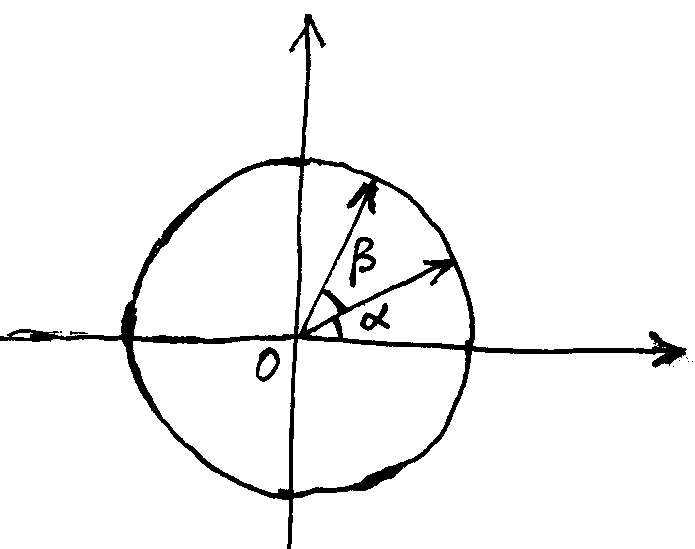
\includegraphics[width=4.5cm]{Preface/alphaplusbeta.png}
%\caption{default}
%\label{default}
\end{center}
\end{figure}


等式左侧(LHS):

\begin{eqnarray*}
(\cos \alpha + i \sin \alpha) \cdot (\cos \beta + i \sin \beta)  \\
 (\cos \alpha \cos \beta - \sin \alpha \sin \beta ) + i ( \sin \alpha \cos \beta + \cos \alpha \sin \beta)
\end{eqnarray*}

等式右侧(RHS):

\begin{equation}
\cos (\alpha + \beta) + i \sin (\alpha + \beta)
\end{equation}

因此:

\begin{eqnarray}
\cos (\alpha + \beta) &=& \cos \alpha \cos \beta - \sin \alpha \sin \beta\\
\sin (\alpha + \beta)&=& \sin \alpha \cos \beta + \cos \alpha \sin \beta
\end{eqnarray}

在物理学中,任何测量值都是一个实数,我们无法从“表盘”中读出个虚数来,但引入虚数,确实可给我们带来计算上的便利。

比如我们经常用$e$指数函数来表示一个波动:

\begin{equation}
\psi (x,t) = A e^{i (kx - \omega t)}
\end{equation}

这里相位是:

\begin{equation*}
k x - \omega t
\end{equation*}

对波动$\psi(x,t) =  A e^{i (kx - \omega t)} $,取固定相位,比如0,研究相位为0传播的速度,这就是相速度(phase velocity)。

\begin{equation*}
 k x  - \omega t = 0
\end{equation*}

对上式做微分,

\begin{equation*}
 k dx - \omega dt  = 0
\end{equation*}

于是得到相速度$v_p$:

\begin{equation}
v_p = \frac{dx}{dt}= \frac{\omega}{k} = \frac{2 \pi / T}{2 \pi / \lambda} = \frac{\lambda }{T }
\end{equation}

这里$v_p > 0$,表示波动是从左向右传播的,即沿着$x$轴的正方向传播。

但假如波函数是如下形式:

\begin{equation}
A \cos (kx + \omega t)
\end{equation}

解出来的$v_p < 0$,我们就说波动是从右向左传播的。


因为虚部的存在,$\psi (x,t)$本身并不直接对应物理量,但$\psi (x,t)$取实部

\begin{equation*}
\Re \psi (x,t) = A \cos (kx - \omega t)
\end{equation*}

就可以对应物理量了。比如机械波的振动,电磁波中电场分量或磁场分量的取值等等。


\subsection{直角坐标系}

我们回到本节一开始的思路,人对运动物体的研究是要借助凝视,或借助高速摄像机的。所谓高速摄像机就是对百万分之一秒($10^{-6}$s),甚至更短的时间间隔进行曝光。

借助于曝光时间很短,但又绝对不是0的高速摄像机,我们可以拍着胸脯说:我已经把我关心的运动都静态化了,或我们已经把它们——运动中的物体——冻结住了。至少可以在高速摄像机里成像了。

然后我们应如何描述它们呢?

物理学家的办法是建立一个坐标系,考虑到真实的世界是三维的,有前后、左右和上下的区别,我们选我们所在的地方为原点,然后以向右为$x$轴,向前为$y$轴,向上为$z$轴,这样我们就得到了一个三维的直角坐标系,也叫笛卡尔坐标系(cartesian coordinate)。笛卡尔(1596 — 1650)是与伽利略几乎同时的一位科学-哲学家。

我们把$x$轴、$y$轴和$z$轴想象为一根长长的尺子,我们需要在尺子上划分刻度,比如以米为单位。物体的位置可以用三个数($x, y, z$)来表示。

首先我们由物体的所在向$z$轴做投影,得到的就是$z$。然后我们由物体的所在出发吊一根铅垂线,得到物体在$x-y$平面上的投影($x, y$),然后再由这一点出发,向$x$轴做垂线,得到的就是$x$,向$y$轴做垂线,得到的就是$y$。

\begin{figure}[htbp]
\begin{center}
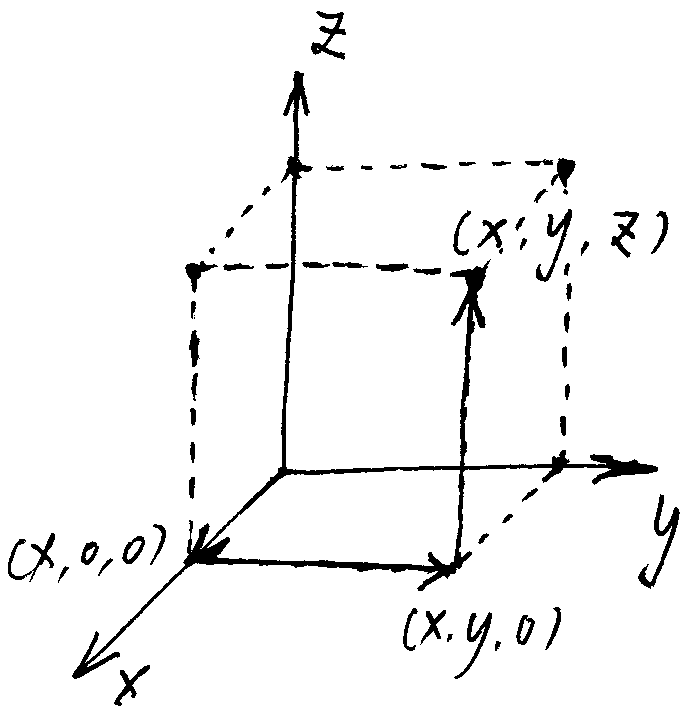
\includegraphics[width=5cm]{Preface/cartesianxyz.png}
%\caption{default}
%\label{default}
\end{center}
\end{figure}

对于大小可以忽略的物体而言,我们说出物体所在的位置,就算交待清楚了。比如:“在$t$等于0秒,物体的$x$取5米,$y$取3米,$z$取0米。”这可能是在描述我家里的玩具小汽车。

这个上下、左右、前后是怎么定的?

我们一般都说物理世界是各向同性的,是平移对称的,即我们在世界的不同地方,不论是巴黎、北京还是纽约,不论我们如何选取我们的坐标轴的取向,我们都会得到相同的物理规律。不同坐标系下,物理陈述的关系可以用一组数学公式描述,这个差不多就是研究相对论的出发点了。

这些当然都对。但我现在想说的是,如果一开始就这么“任意”,我们可能压根就不会得到三维直角坐标系这个概念。

当我们定下第一个三维直角坐标系的时候,上下、左右、前后还是有标准的。

上下:在地球表面上,因为重力的关系,向下落是物体的自然倾向,向上是需要解释的。

前后:人本身并不是前后对称的,眼睛长在脸的前面,所以我们只能向前看,向后看必须要扭脖子。

左右:这个比较难区分,假如你在一个小孩的左侧和右侧放上同样的好吃的,他有可能会真的往左动动,然后又往右,如此纠结、犹豫一番,才会扑向左侧或右侧的好吃东西。难归难,但对人而言,还是有区分左右的标准的,比如对普通人来说,右手会更强健有力一些。

比如我们可以这样:先定上下,用铅垂线;然后定东西,以太阳升起的方向;然后再定南北。或者也可以先定南北,借用北极星的方位。


\subsubsection{单位向量}

在笛卡尔坐标系中,物体的位置用矢量$r$表示,所谓矢量就是一个既有大小,又有方向的量,所谓方向和我们所处的三维空间有关,它来源于我们可以绕过,或跳过障碍物这类日常经验。

为了强调$r$是矢量,我们用符号$\vec r$表示。

我们现在来定义两个矢量的相加,比如:$\vec r_1 + \vec r_2$,它当然还是个矢量,并且应当满足交换律:

\begin{equation}
\vec r_1 + \vec r_2 = \vec r_2 + \vec r_1 = \vec r
\end{equation}

如果是讲数学的话,这就是个规定,不需要再多做解释。但如果是物理的话,我们会再多说几句,说这是先往$\vec r_1$的方向上走了$r_1$远,然后又沿$\vec r_2$方向走了$r_2$远,这么走的效果和先$r_2$再$r_1$的效果是一样的。

这里我们是在替物理挑一套合适的数学语言。这套数学的语言对经典力学而言,具体说是对经典力学里如何描述质点的运动而言,就是三维实系数的矢量空间。

三维实系数矢量空间中的任何一个矢量都可以按照平行四边形的法则进行分解。

\begin{equation}
\vec r = \vec r_1 + \vec r_2
\end{equation}

但有一种分解方式会比较方便,即$\vec r_1$和$\vec r_2$垂直的方式,在这种方式下,我们说$\vec r_1$中没有丝毫的$\vec r_2$的成分,同样$\vec r_2$中没有丝毫$\vec r_1$的成分。

这符合最佳分类的一般原则:

\begin{center}
既不重复,也不遗漏!
\end{center}

在$\vec r_1$方向上的单位向量是:

\begin{equation}
\vec i = \frac{\vec r_1}{r_1}
\end{equation}

在$\vec r_2$方向上的单位向量是:

\begin{equation}
\vec j = \frac{\vec r_2}{r_2}
\end{equation}

\begin{figure}[htbp]
\begin{center}
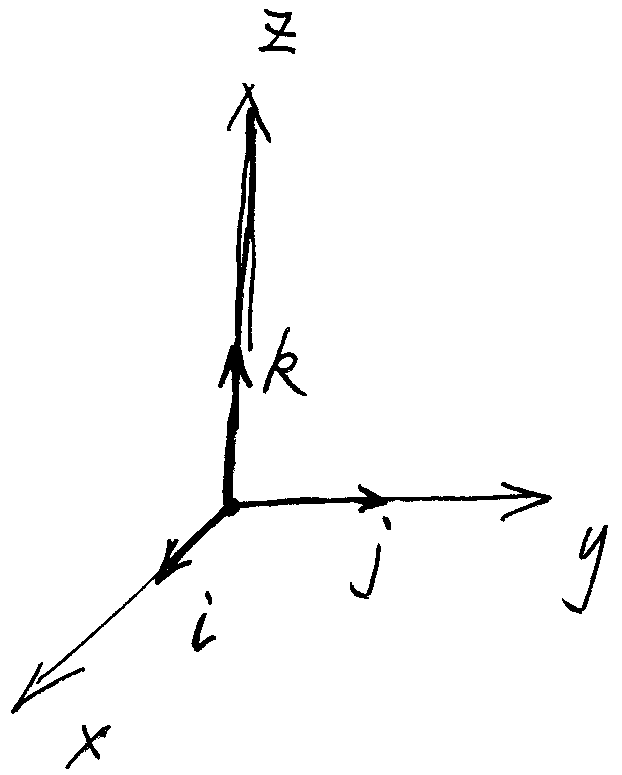
\includegraphics[width=4cm]{Preface/cartesian.png}
%\caption{default}
%\label{default}
\end{center}
\end{figure}

我们选取$\frac{\vec r_1}{r_1}$为$x$方向上的单位向量,记做$\vec i$;选取$\frac{\vec r_2}{r_2}$为$y$方向上的单位向量,记做$\vec j$。最后还剩一个$z$方向上的单位向量$\vec k$,我们通过矢量的叉乘(cross product)得到它。

\begin{equation}
\vec k = \vec i \times \vec j
\end{equation}

叉乘在这里需要满足右手法则,即:

\begin{enumerate}
\item 

伸出右手,除大拇指外其他手指指的方向是$\vec i$的方向;

\item

手指自然向手掌弯曲并握拳,手指弯曲后指的方向是$\vec j$的方向;

\item 

最后大拇指指的方向是$\vec k$的方向。

\end{enumerate}

利用叉乘,我们有更多$\vec i , \vec j , \vec k$的性质:

\begin{eqnarray}
\vec i \times \vec j & = & \vec k \\
\vec j \times \vec k & = & \vec i \\
\vec k \times \vec i & = & \vec j 
\end{eqnarray}

有了$\{ \vec i , \vec j , \vec k  \}$的定义,三维空间中的任何一个矢量$\vec r$都可以表示为$\vec i , \vec j , \vec k$的线性叠加。

\begin{equation}
\vec r =  \vec i  r_i +  \vec j  r_j +  \vec k  r_k 
\end{equation}

这就是说我们的分类(分成$\vec i , \vec j , \vec k$三类)并不遗漏,用数学的术语说,我们的分类是完备的。

\subsubsection{点乘和叉乘}

\begin{enumerate}

\item 

对两个矢量$\vec a, \vec b$,我们可以定义点乘(point product)

\begin{equation}
\vec a \cdot \vec b = a_i b_i + a_j b_j + a_k b_k
\end{equation}

矢量点乘的例子是做功,即“功等于力点乘位移”:

\begin{equation}
W = \vec F \cdot \vec l
\end{equation}

有一点必须提醒大家,因为矢量的记号里的这个箭头 \quad  $\vec {}$ \quad 写起来实在麻烦,所以我们经常会省去,前提是你心里要明白。实际上理论物理学的永恒主题就是发明记号,然后再简化记号。表面看起来很抽象,但其实都是为了方便。

\item

我们可定义矢量$\vec a$的模,即$\vec a$的大小$a$:

\begin{equation}
a = \sqrt{ \vec a \cdot \vec a } = \sqrt{ a_i^2 + a_j^2 + a_k^2 }
\end{equation}

\item

两个矢量$\vec a, \vec b$的叉乘(又叫矢量乘,因为这样乘出来是个矢量):

\begin{equation}
\vec a \times \vec b = 
\left(  
\begin{array} {lcr}
i & j & k \\
a_i & a_j & a_k \\
b_i & b_j & b_k 
\end{array}
\right)
\end{equation}

\end{enumerate}

进一步展开需要用到行列式的知识:

\begin{equation*}
\left(  
\begin{array} {lcr}
i & j & k \\
a_i & a_j & a_k \\
b_i & b_j & b_k 
\end{array}
\right)
= i 
\left(  
\begin{array} {lcr}
 a_j & a_k \\
 b_j & b_k 
\end{array}
\right)
- j
\left(  
\begin{array} {lcr}
 a_i & a_k \\
 b_i & b_k 
\end{array}
\right)
+ k
\left(  
\begin{array} {lcr}
 a_i & a_j \\
 b_i & b_j 
\end{array}
\right)
\end{equation*}

$= \vec i (a_j b_k - a_k b_j) - \vec j (a_i b_k - a_k b_i) + \vec k (a_i b_j - a_j b_i)$

矢量叉乘的例子是力矩$\vec \tau$和角动量$\vec J$等:

\begin{eqnarray}
\vec \tau &=& \vec r \times \vec F \\
\vec J & = & \vec r \times \vec p
\end{eqnarray}


\subsubsection{左手系和右手系}

在物理里面经常会讲左手系和右手系,这个是这样来定的。

伸出你的右手,大拇指向上,剩下的那些手指头做出一个自然向“手掌”握的动作,大拇指的指向是$z$轴的正向,剩下手指头初始指的方向是$x$轴正向,自然握的方向是$y$轴正向。

这样规定的$xyz$坐标系就是右手系,我们在物理里一般都用右手系。

\begin{figure}[htbp]
\begin{center}
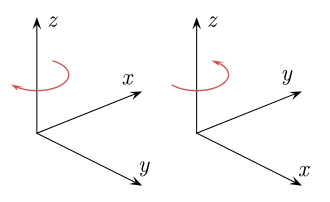
\includegraphics[width=7cm]{Preface/lefthandrighthand.png}
\caption{左图为左手系;右图为右手系。}
%\label{default}
\end{center}
\end{figure}

当然还有左手系(伸出你的左手……),左手和右手的关系好像是照镜子,比如:一个物体在右手系中的坐标是($5, 3, 0$),那么它在左手系中的坐标则可能是($5, -3, 0$)。

对纯平面的东西是没必要分左手和右手的。

比如我拿一张白纸,在纸上画一个向右转的箭头,这个看上去是和向左转的箭头正好相反,但只要你把白纸转过来,你就会发现它其实同时也是个向左转的箭头。

但对三维结构,一个右手的螺旋上升,就没有办法通过一个在三维空间中的重新摆放和定位变成一个左手的螺旋上升。或者更简单的例子:左手握成一个拳头,右手也握成一个拳头,无论我们怎么摆放它们,它们都不可能完全一样。

还是拿一张白纸,我们画一个逆时针旋转的箭头,即面对我们,箭头是向左的,我们再假想这实际上是个三维结构,它是穿过纸面向我运动的。然后我们再把白纸翻转过来,这时固然我们看到的是一个向右转的箭头,或是一个顺时针旋转的箭头,但不要忘记这时这个旋转的箭头已经是穿过纸面远离我运动的了,这就是一个具有右手手性的螺旋。而且随便我们摆放它,这个结构都是个右手手性的螺旋。

DNA双螺旋和蛋白质的$\alpha$螺旋都是有手性的。

\begin{figure}[htbp]
\begin{center}
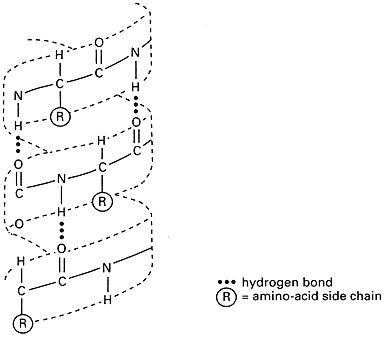
\includegraphics[width=7cm]{Preface/alphahelix.jpg}
\caption{$\alpha$螺旋示意:由于“CO-NH”结构的存在,我们是可以在链上对$\alpha$螺旋定义走向的,它自然是有手性的。}
%\label{default}
\end{center}
\end{figure}


在光学中的例子则是左旋光和右旋光。

\begin{figure}[htbp]
\begin{center}
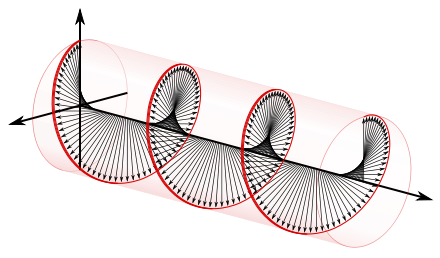
\includegraphics[width=10cm]{Preface/circularpolarization.png}
\caption{按照我们的定义这是一个左旋光}
\label{default}
\end{center}
\end{figure}


\subsection{左旋光和右旋光}

光波就是电磁波,是特定波长(400-700nm)能被我们人眼所见的电磁波,光波传播的方向和光波电分量振荡的方向垂直,光波电分量振荡方向可以是在一个方向上,比如说就固定在$x$方向上,这就是线偏振光,它也可以边振荡边旋转,比如边振荡边往左(或右)转,这就是圆偏振光了。

左旋光或右旋光可以这么定义,假设光是冲着我们传播的,如果电分量是边振荡边向左转就是左旋光,否则就是右旋光。

电磁波是电场$E$和磁场$B$在时间和空间中的传播。它有如下性质:

\begin{enumerate}
\item 

电磁波是横波,电场和磁场振动的方向都和电磁波传播的方向垂直。

电场振动方向$\vec E$,磁场振动方向$\vec B$和电磁波传播的方向$\vec k$,正好构成右手法则。

\item 

根据电磁学的规律。变化的电场会感生变化的磁场,而变化的磁场又会感生变化的电场。

原则上我们只要给出电场$\vec E$随时空的传播,就决定了磁场$\vec B$随时空的传播。

\item

现在我们只需要研究电场$\vec E$随时空的传播。

如果我们选取电磁波传播的方向是$z$轴的正方向的话,电场$\vec E$就在$x-y$平面上。

假如$\vec E$就在$x$轴上,我们说电磁波是$x$-偏振的,因为电磁波就是光波,所以对光来说我们也有$x$-偏振光。

角频率为$\omega$的$x$-偏振光的电场分量就可以表示为:

\begin{equation}
\vec E (z, t) = \vec {e_x} E_0 e^{i ( kz - \omega t ) }  
\end{equation}

这里$\vec {e_x}$表示$x-y-z$坐标系中沿$x$方向的单位矢量。

类似地,我们还可以写出$y$-偏振光的电场分量:

\begin{equation}
\vec E (z, t) = \vec {e_y} E_0 e^{i ( kz - \omega t ) }  
\end{equation}

由于$\vec {e_x}$和$\vec {e_y}$垂直,所以$x$-偏振光里一点$y$-偏振光的成分都没有。反过来说,$y$-偏振光里一点$x$-偏振光的成分都没有。

\item

所谓自然光就是各个方向的偏振光都有,每个方向偏振光的强度都是一样的。

\item

那么圆偏振光如何表达呢?

圆偏振光里面的电场矢量$\vec E$是旋转的,可能向左转,也可能向右转。

$\vec E$在$x$轴的投影:$ \frac{1}{\sqrt{2}} E_0 \cos \theta$

$\vec E$在$y$轴的投影:$ \pm  \frac{1}{\sqrt{2}} E_0 \sin \theta$

如果取正号($\pm$中上面的“+”),($ \frac{1}{\sqrt{2}} E_0 \cos \theta$, $ \frac{1}{\sqrt{2}} E_0 \sin \theta$)正好构成一个向左旋转的圆,或说是逆时针的。(称之为左旋光)

如果取负号($\pm$中上面的“-”),($ \frac{1}{\sqrt{2}} E_0 \cos \theta$, $ - \frac{1}{\sqrt{2}} E_0 \sin \theta$)正好构成一个向右旋转的圆,或说是顺时针的。(称之为右旋光)

考虑到正弦/余弦函数具有如下性质:

\begin{eqnarray*}
\cos (\theta + \pi /2 ) &=& - \sin \theta \\
\cos (\theta -  \pi /2 ) &=& \sin \theta
\end{eqnarray*}

对向左旋转的电矢量,电矢量的$x$分量和$y$分量分别为:

\begin{eqnarray*}
E_x &=& \frac{1}{\sqrt{2}}  E_0 \cos (k z - \omega t) = \frac{1}{\sqrt{2}}  \Re E_0 e^{i (k z - \omega t)}  \\
E_y &=& \frac{1}{\sqrt{2}}  E_0 \cos ( - \pi /2 +  kz - \omega t  ) = \frac{1}{\sqrt{2}}  \Re E_0 e^{ - i \pi /2 } e^{i (kz - \omega t)} \\
{} &=& \frac{1}{\sqrt{2}}  \Re E_0 (-i) e^{i (kz - \omega t)} 
\end{eqnarray*}

类似地,我们可以写出向右旋转的电矢量,表示为:

\begin{eqnarray*}
E_x &=& \frac{1}{\sqrt{2}}  E_0 \cos (k z - \omega t) = \frac{1}{\sqrt{2}}  \Re E_0 e^{i (k z - \omega t)}  \\
E_y &=& \frac{1}{\sqrt{2}}  E_0 \cos ( \pi /2 +  kz - \omega t  ) = \frac{1}{\sqrt{2}}  \Re E_0 e^{ i \pi /2 } e^{i (kz - \omega t)} \\
{} & = & \frac{1}{\sqrt{2}}  \Re E_0 i e^{i (kz - \omega t)} 
\end{eqnarray*}

这么写太啰嗦了,我们把它们写精炼一些,

向右旋转的光:

\begin{equation}
\vec E = \frac{1}{\sqrt{2}} E_0 \Re \left(
\begin{array}{c}
1 \\  i
\end{array}
\right) e^{i (kz - \omega t)}
\end{equation}

简单说电场矢量$\vec E$在$y$方向上的振动比$x$方向上的振动超前$\frac{\pi}{2}$。

向左旋转的光可写为:

\begin{equation}
\vec E = \frac{1}{\sqrt{2}} E_0 \Re \left(
\begin{array}{c}
1 \\ - i
\end{array}
\right) e^{i (kz - \omega t)}
\end{equation}

电场矢量$\vec E$在$y$方向上的振动比$x$方向上的振动要落后$\frac{\pi}{2}$。

类似于$x$-偏振光和$y$-偏振光,向左旋转的光和向右旋转的光也是完全不相容的。

即:左旋光里没有任何右旋光的成分,右旋光里没有任何左旋光的成分。

据说现在3D电影使用的就是左旋光和右旋光,因为用线偏振光有个大毛病,假如左眼看$x$偏振光,右眼看$y$偏振光,我们的脑袋稍微晃一晃,左眼眼镜里偏振片的方向会与$x$方向形成夹角,这样$y$偏振光也能进来一部分了,于是电影的图像就会模糊。

左旋光和右旋光没这个问题,因为它是向左转和向右转的关系,与偏振片本身在空间中的方位无关。所以我们可以让左眼总看到左旋光,而右眼总看到右旋光。


\end{enumerate}

